\chapter{MATLAB Problem 2.1}

In den Abbildungen \ref{fig:2_1_noisefree} bis \ref{fig:2_1_noise_norm} sind die Filterkoeffizienten des
Adaptiven Filters dargestellt. Beim rauschfreien Fall in Abbildung \ref{fig:2_1_noisefree} erkennt man,
dass der Adaptive Filter die Koeffizienten des unbekannten Systems sehr schnell ann�hert. Da kein Rauschen
hinzugef�gt wird, werden diese Koeffizienten sehr gut angeh�hert.

In den Abbiludungen \ref{fig:2_1_noise} und \ref{fig:2_1_noise_norm} ist sehr gut der Unterschied zwischen
NLMS und LMS zu erkennen.

Beim LMS n�hern sich die Koeffizienten etwas schneller als beim NLMS an. Der Grund hierf�r ist, dass beim NLMS
$\mu$ durch die Norm des tapped input Vektors angepasst wird. Bei einer Varianz des Eingangssignals (white noise) von $1$
und einer Filterordnung von 4, wird $\mu$ im Mittel durch 4 dividiert.

Durch das kleinere effektive $\mu$ n�hert sich der NLMS etwas langsamer den Koeffizienten an. Allerdings ist durch das 
kleinere $\mu$ der Excess-Error kleiner (siehe Vorlesung vom 18.11). Somit enthalten die Koeffizienten weniger Fluktuation (weniger Rauschen).
Die Abbildungen \ref{fig:2_1_noise} und \ref{fig:2_1_noise_norm} spiegeln sehr gut die geschilderten
zusammenh�nge wider.
\begin{figure}[ht!]
 \centering
 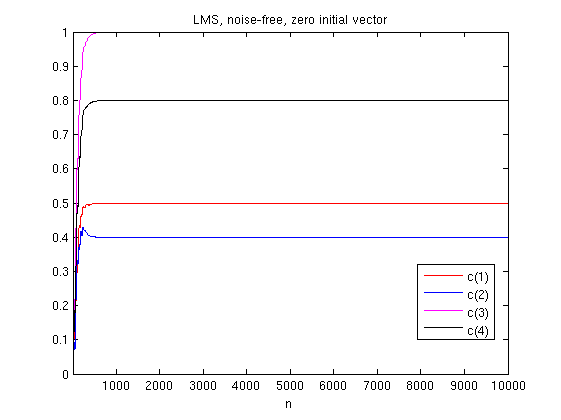
\includegraphics[width=12cm]{./plots/2_1_noisefree.png}
 % 2_3_a_0_0001.png: 560x420 pixel, 90dpi, 15.81x11.85 cm, bb=
 \caption{LMS, $\mu=0.01$, zero-mean white noise input signal with unit variance}
 \label{fig:2_1_noisefree}
\end{figure}


\begin{figure}[ht!]
 \centering
 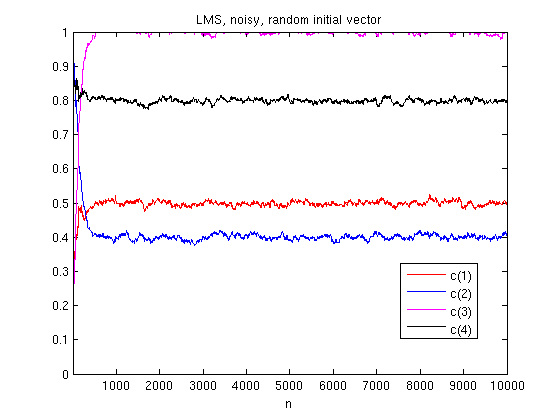
\includegraphics[width=12cm]{./plots/2_1_noise.png}
 % 2_3_a_0_0001.png: 560x420 pixel, 90dpi, 15.81x11.85 cm, bb=
 \caption{LMS, $\mu=0.01$, zero-mean white noise input signal with unit variance, and additional white noise}
 \label{fig:2_1_noise}
\end{figure}


\begin{figure}[ht!]
 \centering
 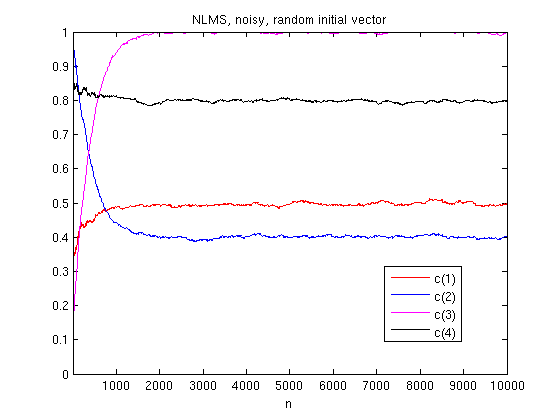
\includegraphics[width=12cm]{./plots/2_1_noise_norm.png}
 % 2_3_a_0_0001.png: 560x420 pixel, 90dpi, 15.81x11.85 cm, bb=
 \caption{NLMS, $\mu=0.01$, zero-mean white noise input signal with unit variance, and additional white noise}
 \label{fig:2_1_noise_norm}
\end{figure}